\section{Полная картина: ширины конструкций АБПР и настоящей работы}\label{sec:extra}

Метод применим и как <<измерительный инструмент>>: для каждой явной решёточной
конструкции из \cite{ABPR} можно вычислить точную ширину $d$ её запрещённого
интервала (в самой работе доказывалось лишь $d\ge1$). Добавим к ним новые
рациональные конструкции настоящей работы. Результаты для $4\le n\le9$
(каждая строка --- оценка $\chi(\R^n,[1,\ell])\le k$ при $\ell<d$; десятичные
значения $d$ округлены вниз):

\begin{center}\small
\begin{tabular}{c c l l l}
\toprule
$n$ & $k$ & решётка / конструкция & $d^2$ & $d$\\
\midrule
4 & 45   & $\Lambda_\star$ (наст. работа) & $^{\dagger}$ & $1{,}016339$\\
4 & 48   & (наст. работа, \S\ref{sec:wide}) & $^{\dagger}$ & $1{,}039657$\\
4 & 49   & $(3+\omega)D_4$ & $7/6$ & $1{,}080123$\\
4 & 54   & $A_4^*$ & $23/20$ & $1{,}072380$\\
5 & 132  & рациональная решётка общего положения (теорема~\ref{thm:r5})
  & $^{\dagger}$ & $1{,}010897$\\
5 & 140  & $A_5^*$, матрица $C_5$ из \cite{ABPR} & $39/35$ & $1{,}055597$\\
6 & 343  & $(3+\omega)E_6^*$ & $7/6$ & $1{,}080123$\\
7 & 1323 & рациональная решётка общего положения (теорема~\ref{thm:r7})
  & $^{\dagger}$ & $1{,}007032$\\
7 & 1372 & $E_7^*$, матрица $C_7$ из \cite{ABPR} & $17/14$ & $1{,}101946$\\
8 & 2401 & $(3+\omega)E_8$ & $7/6$ & $1{,}080123$\\
9 & 17253& $A_9^*$, матрица $C_9$ из \cite{ABPR} & $169/165$ & $1{,}012048$\\
9 & 9604 & ламинирование $E_8/2401$ (\S\ref{sec:dim912}) & $^{\ddagger}$ & $1{,}058126$\\
\bottomrule
\end{tabular}

\smallskip
\begin{minipage}{0.92\textwidth}\footnotesize
$^{\dagger}$~точная дробь $d^2$ громоздка (числитель и знаменатель --- порядка
$30$ десятичных знаков): она равна отношению полей
\texttt{Ddown2}/\texttt{diamup2} файлов \path{audit-data/results/cert45.json}
и \path{audit-data/results/cert48.json} и отношению
\texttt{minimum\_distance\_squared}/\texttt{diameter\_squared} (блок
\texttt{separation}) сертификатов индексов $132$ и $1323$ (\S\ref{sec:r57}).\quad
$^{\ddagger}$~ширина численная (статус \stN); точной рациональной дроби нет.
\end{minipage}
\end{center}

\paragraph{Тождество для эйзенштейновых конструкций.} Для решёток с
$\Z[\omega]$-структурой ($\omega=e^{2\pi i/3}$) и подрешётки
$\Gamma=(3+\omega)\Lambda$ (умножение на $\alpha=3+\omega$, $|\alpha|^2=7$) во
всех проверенных случаях ($n=2,4,6,8$) выполняется точное равенство
\begin{equation}\label{eq:eis}
D\bigl((3+\omega)\Lambda\bigr)^2=\tfrac73\,\lambda_1(\Lambda)^2,
\qquad\text{т.е.}\qquad
d=\frac{\sqrt{7/3}}{\,2R/\lambda_1\,},
\end{equation}
где $R$ --- радиус покрытия. Ширина $d$ зависит \emph{только} от отношения
покрытие/упаковка (рис.~\ref{fig:eis}): при $2R/\lambda_1=\sqrt2$ (решётки
$D_4$, $E_6^*$, $E_8$) получается ровно $d=\sqrt{7/6}$.

Неравенство <<$\ge$>> в~\eqref{eq:eis} мы теперь можем \emph{доказать}, причём
для всех эйзенштейновых решёток сразу; открытым остаётся только вопрос о
равенстве.

\begin{proposition}[планарная нижняя граница]\label{prop:planar}
\textbf{[Т]} Пусть $\Lambda\subset\R^n$ --- решётка с $\Z[\omega]$-структурой.
Тогда для каждого ненулевого $w\in\Lambda$
\[
D\bigl((3+\omega)w\bigr)\ \ge\ \sqrt{7/3}\,\|w\|,
\qquad\text{в частности}\qquad
D\bigl((3+\omega)\Lambda\bigr)\ \ge\ \sqrt{7/3}\,\lambda_1(\Lambda).
\]
\end{proposition}

\begin{proof}
Векторы $\pm w,\ \pm\omega w,\ \pm(1+\omega)w$ лежат в $\Lambda$ и имеют одну
норму $\|w\|$ (умножение на обратимые элементы $\Z[\omega]$ --- изометрия
плоскости $P=\mathrm{span}(w,\omega w)$). Соответствующие шесть полупространств
$\langle x,u\rangle\le\|u\|^2/2$ содержат $V_0$, а их нормали лежат в $P$,
поэтому ортопроекция $\pi_P(V_0)$ содержится в правильном шестиугольнике $H$ ---
ячейке Вороного решётки $\Z[\omega]w\cong A_2$ масштаба $\|w\|$ внутри $P$.
Точка $v/2=(3+\omega)w/2$ лежит в $P$, и
\[
\dist\bigl(v/2,\,V_0\bigr)\ \ge\ \dist_P\bigl(v/2,\,H\bigr)
=\sqrt{7/12}\,\|w\|,
\]
где последнее равенство --- плоская выкладка в $A_2$ (расстояние от точки
$(3+\omega)/2$ до шестиугольника с фасетами на расстоянии $1/2$; оно же ---
известная ширина семицветной раскраски $A_2/7$). Отсюда
$D(v)=2\dist(v/2,V_0)\ge\sqrt{7/3}\,\|w\|$.
\end{proof}

Предложение~\ref{prop:planar} переводит константу $D_{\min}=\sqrt7$ всех
конструкций $(3+\omega)$ настоящей работы ($D_4/49$, $E_6^*/343$, $E_8/2401$ и
горизонтальный пол ламинирования из \S\ref{sec:dim912}) из численно
проверенного факта в теорему: проверка $26\,640$ векторов $E_8$, $2\,466$
векторов $E_6^*$ и $18$ векторов $A_2$ подтверждает повекторное неравенство с
запасом $10^{-11}$ и равенство на минимальных векторах
(\path{audit-data/results/planar_inradius_checks.json}).

Подчеркнём, что сама пороговая константа $\sqrt{7/3}$ здесь не нова: в
замечании~9 работы \cite{ABPR} отмечено, что теорема~3 остаётся верной при
ослабленном условии $2R/\lambda_1\le\sqrt{7/3}\approx1{,}5275$ вместо $3/2$,
но авторы <<не знают решёток, которые использовали бы это усиление>>. Условие
$d\ge1$ в~\eqref{eq:eis} --- это в точности их ослабленное условие; новизна
здесь в другом: равенство~\eqref{eq:eis} даёт не только порог, но и \emph{точную}
ширину интервала для каждой конкретной решётки, а таблица выше как раз и
предъявляет решётки, реализующие усиление.

У решётки Лича $\Lambda_{24}$ отношение $2R/\lambda_1$ также равно $\sqrt2$, и
классическая оценка $\chi(\R^{24})\le7^{12}$ уже доказана в \cite{ABPR}
(там $7^{n/2}$ получено для $n\in\{6,8,24\}$). Предложение~\ref{prop:planar}
добавляет к ней \emph{ширину}: поскольку для нижней границы $D\ge\sqrt{7/3}\,
\lambda_1$ равенство в~\eqref{eq:eis} не требуется,
\[
\chi\bigl(\R^{24},[1,\ell]\bigr)\le7^{12}\qquad(\ell<\sqrt{7/6}\,)
\]
--- теперь строгий результат, а не гипотеза. Для решётки Коксетера--Тодда
$K_{12}$ имеем $2R/\lambda_1=\sqrt{8/3}\approx1{,}633>\sqrt{7/3}$, и
формула~\eqref{eq:eis} даёт $d=\sqrt{7/8}\approx0{,}935<1$ --- конструкция
теоремы~3 из \cite{ABPR} на $K_{12}$ не проходит даже в усиленной форме
замечания~9 (частичный отрицательный ответ на их открытый вопрос~2). В
\S\ref{ssec:dim912neg} тот же вывод получен и для комплексного ранга~$5$
(размерность~$10$), где наилучшая эйзенштейнова решётка даёт
$2R/\lambda_1=\tfrac23\sqrt7\approx1{,}7638$.

\begin{figure}[t]
\centering
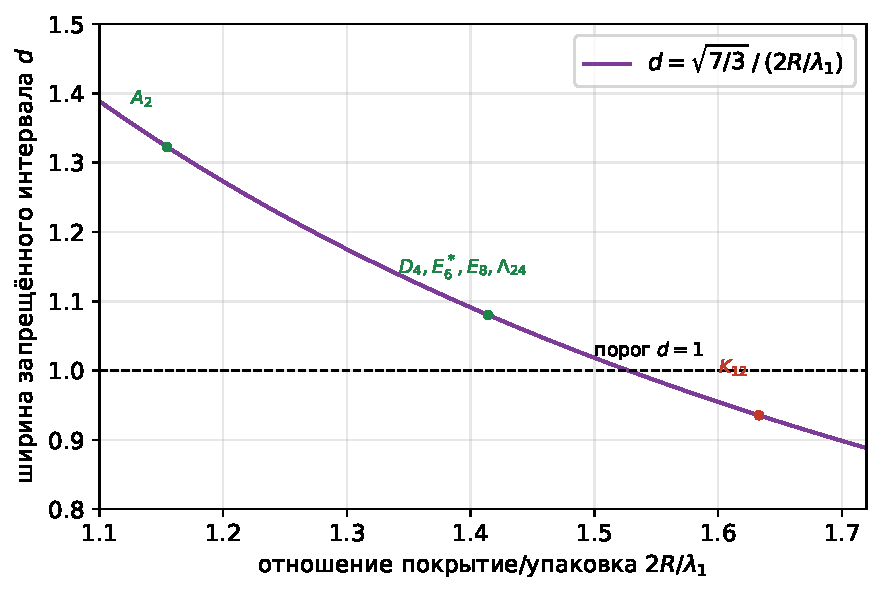
\includegraphics[width=0.6\textwidth]{fig_eisenstein.pdf}
\caption{Тождество~\eqref{eq:eis}: ширина $d$ эйзенштейновой конструкции против
отношения покрытие/упаковка $2R/\lambda_1$. Проверенные решётки $D_4,E_6^*,E_8$
(все с отношением $\sqrt2$) дают ровно $d=\sqrt{7/6}$; для $\Lambda_{24}$
нижняя граница ширины теперь доказана (предложение~\ref{prop:planar}), а для
$K_{12}$ ширина падает ниже порога.}
\label{fig:eis}
\end{figure}

\paragraph{Оптимальность конструкции $C_5$ на фиксированной $A_5^*$.}
Исчерпывающим перебором \emph{всех} $1\,424\,115\,231$ подрешёток
индекса~$140$ решётки $A_5^*$ установлено, что явная конструкция $C_5$ из
\cite{ABPR} оптимальна на этом индексе и по ширине:
$\max d=\sqrt{39/35}$. Теорема~\ref{thm:r5} этому не противоречит: она меняет
родительскую форму и использует индекс~$132$.


